\chapter{Análisis sintáctico}
\section{¿Qué es un analizador sintáctico?}
Un analizador \textbf{sintáctico} (o parser) es un programa informático que analiza una cadena de símbolos de acuerdo a las reglas de una gramática formal. El término proviene del latín \textit{pars}, que significa parte (del discurso). Usualmente hace parte de un compilador, en cuyo caso, transforma una entrada en un árbol sintáctico de derivación.
\section{Función del analizador sintáctico}
Las funciones del analizador sintáctico son las siguientes:
\begin{itemize}
	\item Analizar la secuencia de tokens y verificar si son correctos sintácticamente.
	\item Obtener una representación interna del texto fuente.
	\item Avisar de los errores sintácticos detectados.
\end{itemize}
\begin{figure}[h]
	\centering
	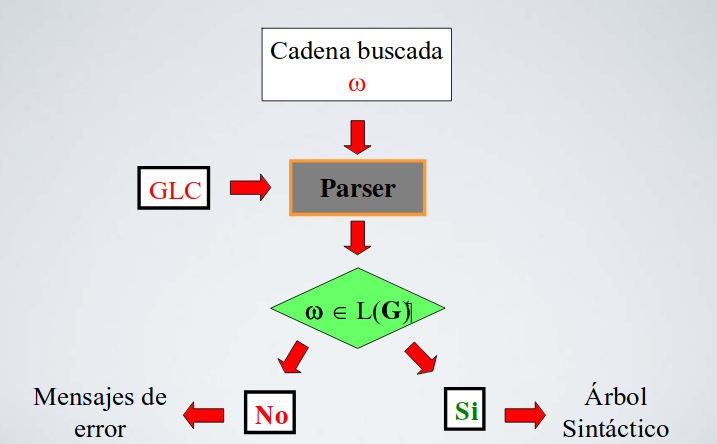
\includegraphics[width=0.7\linewidth]{img/11}
	\caption{Analizador sintáctico}
	\label{fig:5}
\end{figure}
\clearpage
\subsection{Ejemplo funcionamiento}
\begin{figure}[h]
	\centering
	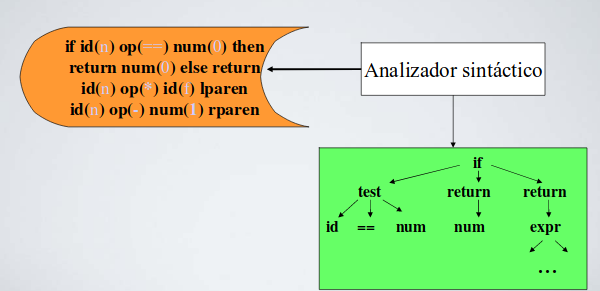
\includegraphics[width=0.7\linewidth]{img/ejemplo_sintactico}
	\caption{}
	\label{fig:ejemplosintactico}
\end{figure}

\textbf{¿Qué necesitamos para poder realizar el análisis sintáctico?}
\newline
Mecanismo para describir las sentencias válidas del lenguaje fuente.
Un sistema que decida ante una entrada ( un programa en texto fuente) si es correcto sintácticamente o no.
\newline
Alguna representación sintáctica del programa.
\newline
\textbf{¿Por qué no se utiliza la misma construcción que en el Analizador Léxico? ¿Por qué no utilizamos AFD's para este tipo de situaciones?}

Porque describir estructuras del tipo $a^nb^n$ usando expresiones regulares es \textbf{imposible}, Lema de Bombeo.
\newline
\newline
\textbf{¿Solución?}

\begin{itemize}
	\item Empleo de construcciones recursivas
	\item Empleo de Gramáticas Libres de Contexto o GLC
\end{itemize}


\section{Gramáticas libres de contexto}

Una gramática libre de contexto se define como la cuádrupla	$G =(V,T,P,S)$
	\begin{itemize}
		\item V: símbolos no terminales de la gramática.
		\item T: símbolos terminales de la gramática.
		\item P, producciones de la gramática.
		\item S, símbolo inicial de la gramática.
	\end{itemize}
Sus producciones P, son de la forma:
\newline
\begin{center}
	$A\Rightarrow\alpha$, donde A$\epsilon$V y $\alpha\epsilon$(V$\cup$T)+
\end{center}
Generalmente se permiten producciones nulas:
\begin{center}
	$A\Rightarrow\epsilon$
\end{center}
\section{Derivación}
El proceso de derivación descrito informalmente consiste en :
\begin{itemize}
	\item Comenzar con el símbolo inicial de la gramática, "S", como cadena de entrada.
	\item Seleccionar un símbolo no-terminal N en la cadena y una producción $N\Rightarrow s_1...s_k$ y cambiar la N por $s_1...s_k$ en la cadena.
	\item Repetir el paso 2, hasta que tengamos una cadena \textbf{w} formada únicamente por símbolos terminales, entonces decimos que \textbf{w} es una cadena generada por la gramática.
\end{itemize}
Principalmente hay dos tipos de derivación:
\begin{itemize}
	\item Derivación más a la izquierda
	\item Derivación más a la derecha
\end{itemize}
Si siempre se sustituye en símbolo terminal más a la izquierda tendremos el primer caso, por el contrario, si es sustituido el más a la derecha tendremos el segundo caso.
\section{Árboles sintácticos}
Un \textbf{árbol sintáctico} es una representación gráfica de las derivaciones realizadas hasta obtener una cadena.
\begin{figure}[h]
	\centering
	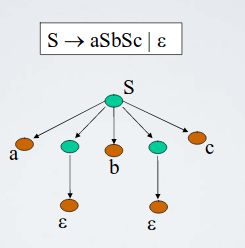
\includegraphics[width=0.5\linewidth]{img/treee}
	\caption{}
	\label{fig:treee}
\end{figure}
\begin{itemize}
	\item Raíz: símbolo inicial de la gramática.
	\item Nodos interiores: símbolos no terminales.
	\item Nodos hojas: símbolos terminales.
\end{itemize}
Cada Nodo interior tendrá como hijos, la parte derecha de la producción aplicada en nodos, ordenados de izquierda a derecha.
\section{Ambigüedad}
Una gramática es \textbf{ambigua} si hay al menos una sentencia que se pueda generar mediante dos o más arboles distintos.
\newline
\newline
Un lenguaje generado por una gramática ambigua es una lenguaje ambiguo.
\newline
\newline
Si todas las gramáticas que generan un determinado lenguaje son ambiguas entonces se dice que el lenguaje es un \textbf{lenguaje inherentemente ambiguo}. 
\newline
\newline 
Nosotros tenemos que trabajar con lenguajes no inherentemente ambiguos.
\newline
\newline
Los analizadores sintácticos deben trabajar con gramáticas no ambiguas.
\section{Estrategias de análisis sintáctico}
\section{Tratamiento de error}
\section{Notacion BNF y EBNF}


